\chapter{Constraint solvers}

\section{\eclipse}

\subsection{Description}

\eclipse is open source constraint satisfaction solving system based on Prolog 
programming language. It is available for Microsoft Windows NT family, 
Linux 32bit/64bit, MacOS and SunOS Sparc platforms. The system is based on the Prolog programming
language which is extended bz new predicates and operators. Prolog extensions are 
more described in "Modelling Capabilities" subsection. In general it can be said that \eclipse
system tends to be SICStus Prolog compatible. \eclipse provides grafical interface,
methods to communicate with hosting operating system or via network. 

As stated in \cite{wiki:Eclipse} \eclipse is developed until 1995 at the European 
Computer-Industry Research Centre in Munich and then until 2005 at the Centre for 
Planning and Resource Control at Imperial College London. It is currently copyrighted by 
Cisco Systems. In September 2006, it was released as open source software under 
the Cisco Systems|Cisco-style MPL, equivalent to the Mozilla Public License.

In the time of writing this thesis it is available in version 5.10 which is benchmarked.


\subsection{Modelling capabilities}

** TO BE WRITTEN **

\subsection{Programming support features}

** TO BE WRITTEN **


\section{SICStus Prolog}

\subsection{Short description}

** TO BE WRITTEN **

\subsection{Modelling capabilities}

** TO BE WRITTEN **

\subsection{Programming support features}

** TO BE WRITTEN **


\section{Gecode}

\subsection{Short description}

** TO BE WRITTEN **

\subsection{Modelling capabilities}

** TO BE WRITTEN **

\subsection{Programming support features}

** TO BE WRITTEN **


\section{Choco}

\subsection{Short description}

Choco is java library for solving CSP distributed as jar archive. Therefore it can
be used in every Java program which allows easily integrate CSP solver to applications.
Project is available at Sourceforge where user can found sources, documentation (in 
JavaDoc and wiki system with several tutorials) and binaries (compiled jar archive).

Beacuse Choco is is Java library, it does not need its own IDE and compiler. User can
use for example Eclipse IDE or other java development tool by his preference.

Authors are now developing Choco2 which is going to supress Choco but in time of 
writing of this thesis Choco2 is still under development.

\subsection{Modelling capabilities}

Choco 

\subsection{Programming support features}

** TO BE WRITTEN **

\section{Mozart}

\subsection{Short description}

Mozart is CSP solver implementing programmin language Oz. Oz contains most of the 
concepts of the major programming paradigms, including logic, functional (both 
lazy and eager), imperative, object-oriented, constraint, distributed, and 
concurrent programming. In addition to multi-paradigm programming, the major 
strengths of Oz are in constraint programming and distributed programming.

Mozart uses as its interface Emacs editor which is customized for oz files.  

\subsection{Modelling capabilities}

** TO BE WRITTEN **

\subsection{Programming support features}

Mozart provides unique tool {\em Mozart Explorer} (screenshot is in figure \ref{mozart-explorer-screenshot}

\begin{figure}
\caption{\label{mozart-explorer-screenshot}Mozart Explorer}
\begin{center}
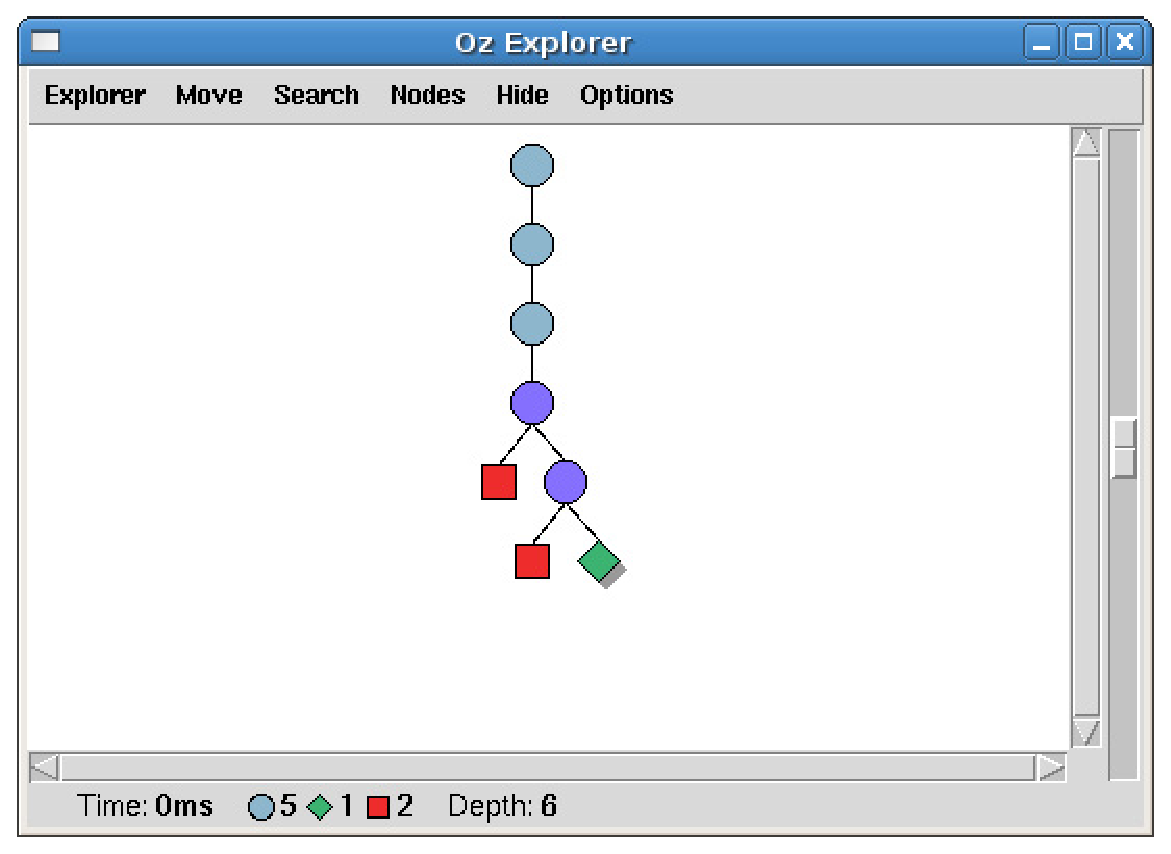
\includegraphics[height=5cm]{images/screenshoty/explorer.eps}
\end{center}
\end{figure}

\begin{figure}[b]
\begin{minipage}[t]{5.0cm}
\caption{\label{srq-mozart-folded}Mozart Explorer -- solution of SRQ in folded version}
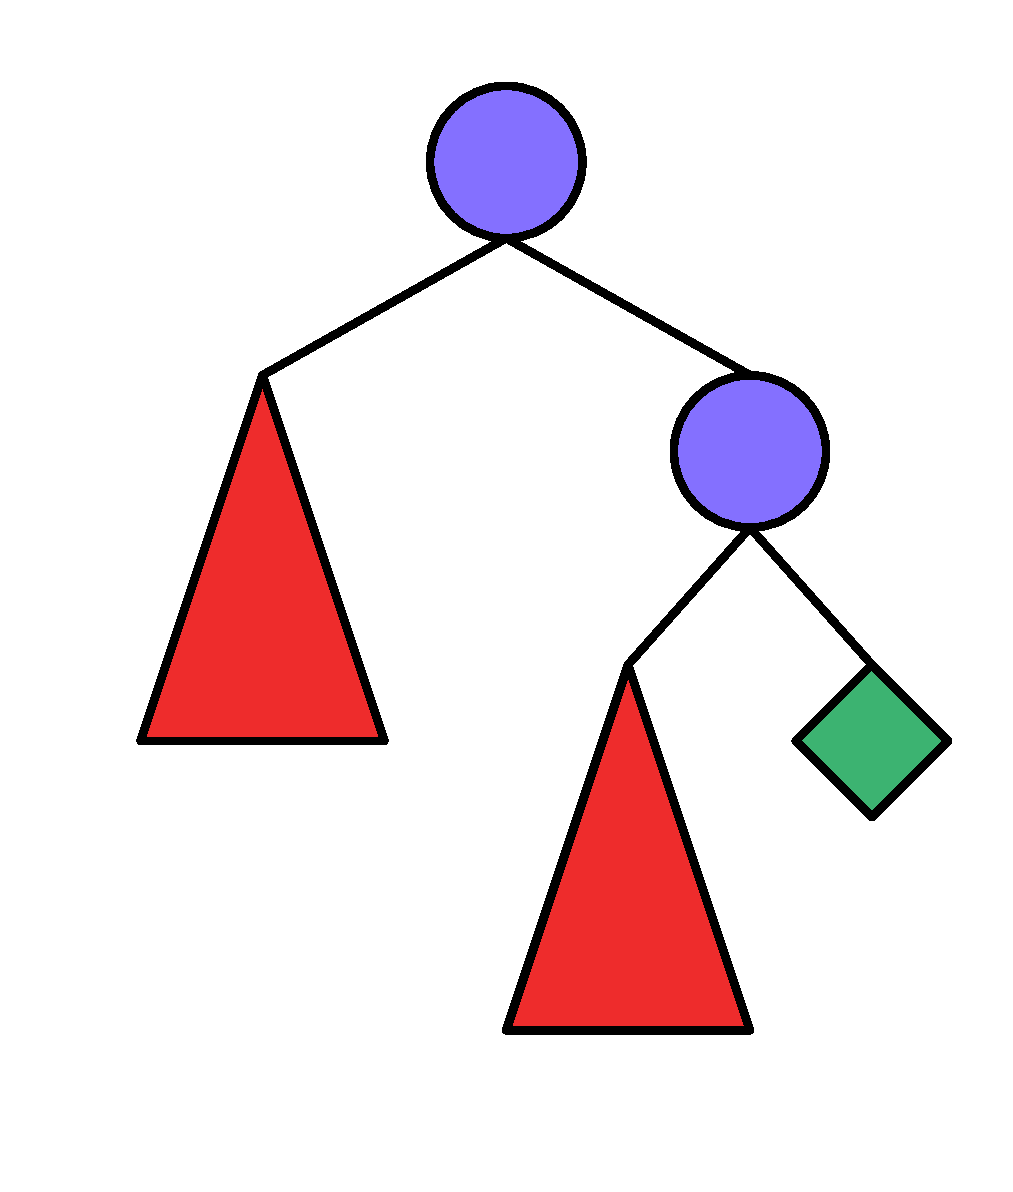
\includegraphics[height=5cm]{images/mozart/srq.oz.color.folded.eps}
\end{minipage}
\hfill
\begin{minipage}[t]{6.0cm}
\caption{\label{srq-mozart-unfolded}Mozart Explorer -- solution of SRQ in unfolded version}
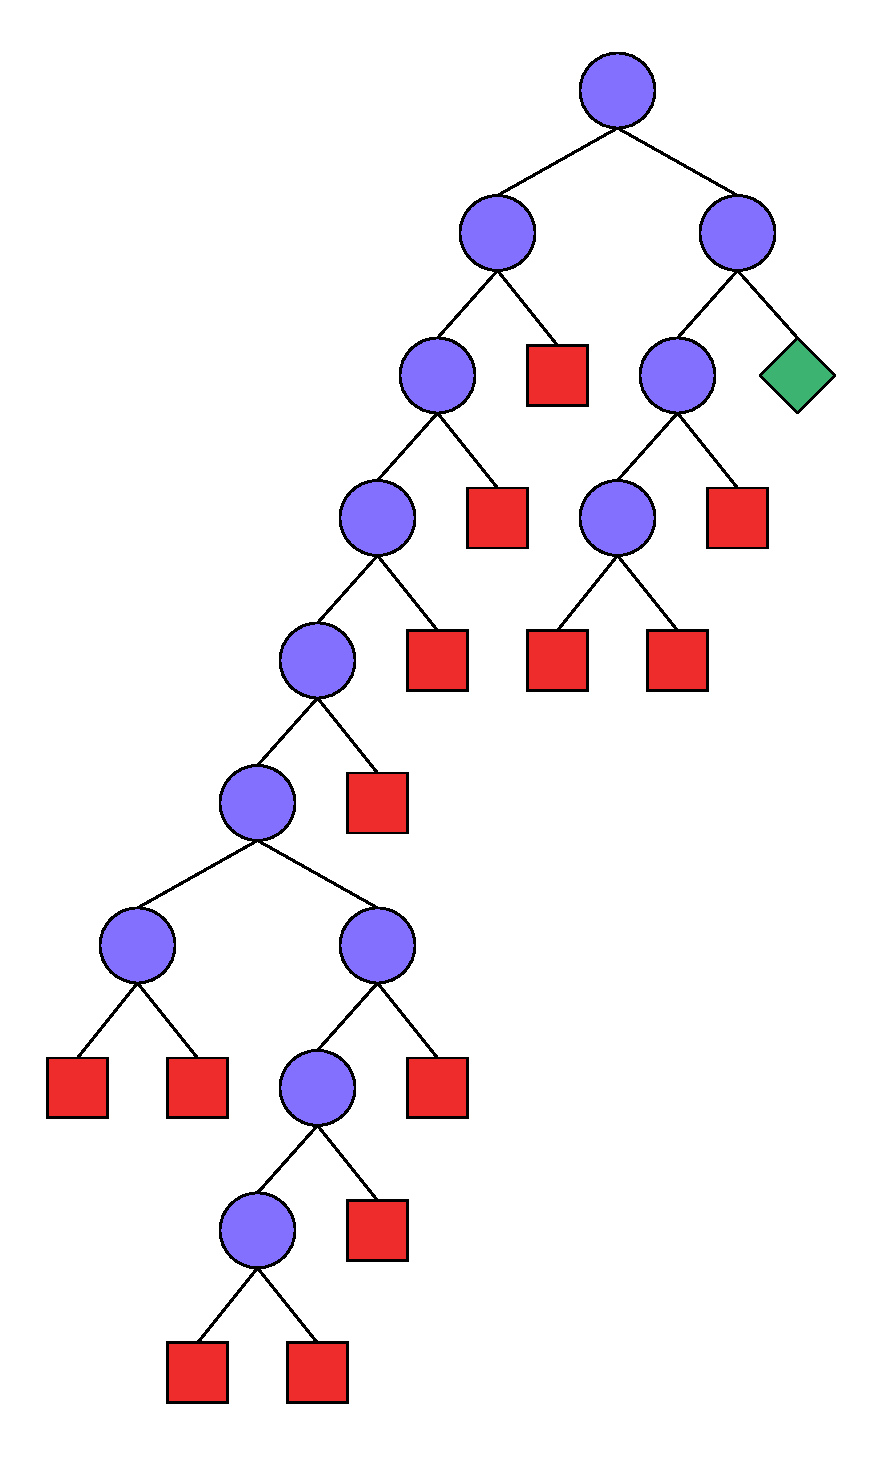
\includegraphics[height=8cm]{images/mozart/srq.oz.color.unfolded.eps}
\end{minipage}
\end{figure}


\section{Minion}

\subsection{Description}

Minion is very low level CSP system with strictly limited set of commands. One 
can describe programming in minion as "constraint satisfaction machine language".
As an example we can demonstrate in on the 4-queens problem.

Common description is:

\begin{align}
\forall i,j, i \neq j & : Q_i \neq Q_j \\
\forall i,j, i < j & : | Q_i - Q_j | \neq j - i 
\end{align}

However in minion there has to be twelve auxiliary variables. Minion does not 
support "sum is equal". If user want to achieve "sum is equal" constraint it has 
to be modified from


Also there is nothing like for or while cycles, whole problem has to be defined in
the input file, which makes programming in pure minion really difficult and nearly
impossible to scale because of growing of auxiliary variables.

The 4-queen problem then looks as follows

\begin{equation*}
\begin{gathered}
Q_2 - Q_3 \leq a_0 \\
Q_1 - Q_3 \leq a_2 \\
Q_1 - Q_2 \leq a_4 \\
Q_0 - Q_3 \leq a_6 \\
Q_0 - Q_2 \leq a_8 \\
Q_0 - Q_1 \leq a_{10}
\end{gathered} \qquad \begin{gathered}
Q_2 - Q_3 \geq a_0 \\
Q_1 - Q_3 \geq a_2 \\
Q_1 - Q_2 \geq a_4 \\
Q_0 - Q_3 \geq a_6 \\
Q_0 - Q_2 \geq a_8 \\
Q_0 - Q_1 \geq a_{10}
\end{gathered} \qquad \begin{gathered}
| a_0 | = a_1 \\
| a_2 | = a_3 \\
| a_4 | = a_5 \\
| a_6 | = a_7 \\
| a_8 | = a_9 \\
| a_{10} | = a_{11}
\end{gathered} \qquad \begin{gathered}
a_{11} \neq 1 \\
a_9 \neq 2 \\
a_7 \neq 3 \\
a_5 \neq 3 \\
a_1 \neq 1 \\
\text{alldifferent}(Q_1,Q_2,Q_3,Q_4)
\end{gathered}
\end{equation*}

As one can see, the problem is described strictly for four queens variant. If there is 
need to extend number of queens whole problem description has to be rewriten.

Fortunately there exists java program Tailor by Andrea Rendl. Tailor converts program
written in Essence' programming language to input format of Minion. Essence' is solver
independent language which describe CSP. More information about this programming language
can be found in \cite{constraints:essence}. Essence' defines syntactic sugar constructions
like \verb=forall= (abbreviation for $a_1 \mand a_2 \mand a_3 \mand \dots$), 
\verb=exists= (abbreviation for $a_1 \mor a_2 \mor a_3 \mor \dots$), \verb=sum= and others.

Great advantage compared to standard Minion input is possibility to scale problems
with given variable. In Minion, the input file can specify for example 4-queens problem 
but for other number of queens is the file unuseful. Programs in Essence' can be written
using constants which are substituted during translation to Minion input format.
As an example of Essence' program we will show 4-queens problem in figure \ref{essence-source-4queens} 
on page \pageref{essence-source-4queens}.  

\begin{figure}
\caption{\label{essence-source-4queens}Example of 4-queens program in Essence'}
\begin{verbatim}
language ESSENCE' 1.b.a

find queens: matrix indexed by [int(1..n)] of int(1..n)

such that

forall i: int(1..n). forall j: int(i+1..n).

  | queens[i] - queens[j] | != | i - j |,

  alldiff(queens)
  
letting n to be 4
\end{verbatim}
\end{figure}

During translation Tailor normalize Essence' program then converts it to flat Essence'.
Flat Essence' is programm in essence which does not contain any syntactic sugar structures.
This program is then converted to Minion input format.

Tailor is written in Java and is distributed as JAR package. It provides graphic interface
with editor of Essence' code. User can directly convert program in Essence' to Minion
and then run it and see the result if any. Tailor can be also used as non-interactive 
tool which only converts from Essence' to Minion.

\subsection{Modelling capabilities}

Minion can evaluate constrained variables of types {\em bool}, {\em discrete}, {\em bound} 
and {\em sparsebound}. Bool variable has $\{0,1\}$ domain with special 
optimised data structure which provides better performance. Domain of discrete variable is 
range of integers. Memory usage and worst-case performance of most operations
is $O(\text{domain size})$. Discrete domain variable can represent any
subset of domain. Bound variable has domain consisting of range of integer.
In contrast to discrete variable the variable can be only reduced by 
changing one of its bounds. Memory and wors-case performance of all 
operations is $O(1)$   Finally sparsebound variable is identical to 
bound variable with exception that domain is an arbitrary range of 
integers. Further description of variable types and performance of 
their using can be found in \cite{minion-manual}. The variables can
form matrices, vectors and tensors (matrices with more dimensions).
Minion provides acces to whole row/column of matrix using syntax 
\verb=q[5,_]= which means "all values of row 5 of matrix $q$".

Minion does not permit nesting of constraints or array indexes. If user 
needs constraints in form \verb=eq(abs(a),6= he must introduce new auxiliary
variable and declare \verb=abs(a, aux) eq(aux,6)=. Also there is no constraint
stating $\sum{a_i} = b$. One must declare $\sum{a_i} \leq b$, $\sum{a_i} \geq b$.
These facts makes practical programming in Minion really hard because 
number of auxiliary variables grows very fast. However user still can 
use Tailor to generate input file for Minion.

Result can be simply solution of the CSP or maximisation/minimisation of
some given variable. 

Minion is not suitable for non-integer variables. If 
there is no possible remapping to integers -- for example set $\{dog, cat, 
horse\}$ to $\{0,1,2\}$ or range 0.5 to 1.5 in 1 digit precision to range
5 to 10 even authors of Minion recommends to use different solver (\cite{minion-sf-gentian}).

Minion 

  

\subsection{Programming support features}

Minion is low level black-boxed system which means that there is 
not wide support for user. User can print out log of the 
parsing process. This log contains detailed information about loading 
of variables and could help find problem in the input file. Second 
debugging feature which is built in the minion is possibility of 
printing whole decision tree. This log contains listing of all nodes 
and decisions. Following listing is example of decision tree of 
the 4-queens problem.

{\small
\begin{verbatim}
Node: 0,<{1,2,3,4},{1,2,3,4},{1,2,3,4},{1,2,3,4},{-3,-2,-1,0,1,2,3},
{0,2,3},{-3,-2,-1,0,1,2,3},{0,1,3},{-3,-2,-1,0,1,2,3},{0,2,3},
{-2,-1,0,1,2},{0,1,2},{-3,-2,-1,0,1,2,3},{0,1,3},{-3,-2,-1,0,1,2,3},
{0,2,3}>

Node: 1,<{1,2,3,4},{1,2,3,4},{1,2,3,4},{1,2,3,4},{-3,-2,-1,0,1,2,3},
{0,2,3},{-3,-2,-1,0,1,2,3},{0,1,3},{-3,-2,-1,0,1,2,3},{0,2,3},
{-2,-1,0,1,2},{0,1,2},{-3,-2,-1,0,1,2,3},{0,1,3},{-3,-2,-1,0,1,2,3},
{0,2,3}>

SearchAssign:AnyVarRef:LongRange0 = 1

Node: 2,<1,{3,4},{2,3,4},{2,3},{-1,0,1,2},{0,2},{0,1},{0,1},
{-1,0,1,2},{0,2},{-2,-1},{1,2},{-3,-2,-1},{1,3},{-3,-2},{2,3}>

SearchAssign:AnyVarRef:LongRange1 = 3
SearchAction:bt
SearchAssign:AnyVarRef:LongRange1 != 3
SearchAction:bt
SearchAssign:AnyVarRef:LongRange0 != 1

Node: 3,<{2,3,4},{1,2,3,4},{1,2,3,4},{1,2,3,4},{-3,-2,-1,0,1,2,3},
{0,2,3},{-3,-2,-1,0,1,2,3},{0,1,3},{-3,-2,-1,0,1,2,3},{0,2,3},
{-2,-1,0,1,2},{0,1,2},{-2,-1,0,1,2,3},{0,1,3},{-2,-1,0,1,2,3},
{0,2,3}>

SearchAssign:AnyVarRef:LongRange0 = 2

Node: 4,<2,{1,3,4},{1,3},{1,3,4},{-3,-2,-1,0,1,2},{0,2,3},
{-3,-2,-1,0,1,2,3},{0,1,3},{-2,-1,0,1,2,3},{0,2,3},{-2,-1,0,1},
{0,1,2},{-1,0,1},{0,1},{-2,-1,0,1},
{0,2}>

SearchAssign:AnyVarRef:LongRange1 = 1
SearchAction:bt
SearchAssign:AnyVarRef:LongRange1 != 1

Sol: 2 4 1 3
\end{verbatim}
}

Minion does not offer public include headers and library to use the solver
as CSP subsystem in wider C++ application. However examining of source codes
revealed, that minion sources could be used in such way. *** UVIDIME 
VYSLEDEK DOTAZU NA AUTORY ***.
